\documentclass[]{article}
\usepackage{float}
\usepackage{csvsimple}
\usepackage{graphicx} % Required for inserting images
\usepackage{array}
\usepackage{multirow,multicol}
\usepackage{adjustbox}
\usepackage{caption}

%opening
\title{Analysis of Air Quality in London}
\author{S18840}

\begin{document}

\maketitle

\vspace{50pt}
\begin{abstract}
	
	Air quality monitoring is crucial in understanding the environmental conditions that influence public health. Using this report we attempt to analyze the air pollution in London City throughout the year 2022.
	
	The significance of air quality monitoring lies in its direct correlation with public health. Poor air quality is leads to respiratory and cardiovascular diseases, making it important to Gain an understanding of the atmosphere pollutant concentrations in the city that you are most associated with.This report hope to highlight the crucial areas with elevated risk levels and the patterns in pollutant concentrations to undertake effective public health actions.
	
	By providing a comprehensive analysis of air quality parameters, this study hope to contributes to the higher understanding of the impact of air pollution on public health in London City. The findings aim to inform responsible authority and the general public about the critical need for taking measures to improve air quality and safeguard the well-being of city's residents
	
\end{abstract}

\pagebreak

\section*{Introduction}

In the City of London, this study aims to understand the composition of the city's air. Using data collected from 36 well known sites in the city of London from January 1, 2022, to December 31, 2023 using this data we are going to explore the trends in air quality of the City of London.

Our goal is to understand the patterns within London's air quality to achieve that we are gonna use The "London local data 2022" and "London Local sites" data sets as our guide,  those detailing hourly measurements of pollutants like 

\begin{itemize}
	\item $Nitrogen Oxides (NO_x)$  which is a collective term for NO and $NO_{2}$, and its emissions have implications for air quality and environmental health.

  	\item	$SO_2$ emissions, often originating from burning fossil fuels, can lead to respiratory problems and contribute to acid rain.
  	\item$O_3$ While ozone high in the atmosphere is beneficial, ground-level ozone is a pollutant affecting respiratory health and vegetation.
  	\item$PM10$ includes inhalable particles, often originating from industrial activities and traffic emissions, impacting respiratory health
    \item$PM2.5$ consists of fine particles that can penetrate deep into the lungs, posing health risks and contributing to visibility issues 
\end{itemize}

There are total of 36 sites as mentioned in the above but due to various reasons selected pollutants are measured in selected sites.Following are the pollutant gases which we are gonna use as our parameters through out our report and no of sites which data were provided to calculate the composition of these gases

\begin{table}[H]
	\centering
	\csvautotabular{parameter_counts.csv}
	\caption{pollutants and no of sites each pollutant measured}
	\label{tab:parametercounts}
\end{table}


we were provided with the details of these 36 sites,

\begin{itemize}
	\item identification code of the site
	\item name of the site
	\item latitude of the site
	\item longitude of the site
	\item name of the substance measured
\end{itemize}

\pagebreak

Here are the 36 sites that used to collect emission data of each Pollutant

\begin{table}[H]
	\centering
	\csvautotabular{unique_sites.csv}
	\caption{36 sites used in the study}
	\label{tab:sitedetails}
\end{table}


\pagebreak

\section*{Analysis}

\vspace{12pt}

\subsection*{Emission of gases in the year 2022}

if we calculated the total sum of the pollutants that released to the air in the year 2022 through these 36 sites,

\begin{figure}[H]
	\centering
	\includegraphics[width=0.9\textwidth]{Graphs/yearly_graph_1.eps}
	\caption{Total emission of gasses in 2022}
	\label{fig:yearly gases}
\end{figure}

You can see that $NO_2$ is the pollutant which was released in the highest amount, while $NO$ takes second place, and $SO_2$ is the pollutant which is released in the minimum amount.


\pagebreak
\subsection*{Emmission of gases monthly in the year 2022}

If we further investigate to determine the time of the year when these gases are emitted the most,

\begin{figure}[H]
	\centering
	\includegraphics[width=0.9\textwidth]{Graphs/Total_per_month_by_gas_2.eps}
	\caption{Emmission of gases monthly in the year 2022}
	\label{fig:monthly gases }
\end{figure}

You can observe that the months of January, March, and December have the highest sum of pollutant emissions, while the months in the middle of the year have a slightly lower sum of pollutants compared to the beginning and the end of the year. While june registering the lowest amount of pollutant emission

\begin{figure}[H]
	\centering
	\includegraphics[width=0.9\textwidth]{Graphs/Total_per_month_by_gas_3.eps}
	\caption{Emmission of gases monthly in the year 2022}
	\label{fig:seperate monthly gases }
\end{figure}

Using this graph, we can confirm the above theory that middle months have lower emission rates compared to the beginning and end of the year. Additionally, from this graph, you can observe that all pollutants exhibit this pattern, while PM10, PM2.5, and $SO_2$ show more consistent emissions throughout the year.

\pagebreak

\subsection*{Emission of gasses based on sites}
\vspace{12pt}
\underline{{\large Analysis of $NO_2$}}

\vspace{12pt}
As the highest emitted gas in the 2022 lets take a closer look at emission of $NO_2$ based on cities,

\begin{figure}[H]
	\centering
	\includegraphics[width=1\textwidth]{Graphs/no2_by_site_graph.eps}
	\caption{Emission of $NO_2$ based on City}
	\label{fig:no2.1 }
\end{figure}

We can see that Westminster City has the highest emission of $NO_2$ in the year 2022, while other cities have marginally lower values compared to Westminster.


Let's look further into Westminster City. According to the provided data, 

\begin{figure}[H]
	\centering
	\includegraphics[width=1\textwidth]{Graphs/no2_by_Westminister_graph.eps}
	\caption{Emission of $NO_2$ in the city Westminster}
	\label{fig:no2.2 }
\end{figure}

there are seven sites used to calculate $NO_2$ emissions in Westminster City. As shown below, we can observe that all seven sites fall within the range of 200k to 400k. Therefore, authorities should investigate Westminster City to understand the reasons behind the high $NO_2$ emissions.finally we should look into City map of $NO_2$ emissions

\begin{figure}[H]
	\centering
	\includegraphics[width=1\textwidth]{Graphs/No2_map.eps}
	\caption{London map based on $NO_2$ emissions }
	\label{fig:no2.3 }
\end{figure}

Here you can see that $NO_2$ emission is spread out throughout the city. Even though Westminster has the highest emission rates, there aren't any discernible patterns on the map; they are randomly spread throughout.
\pagebreak

\vspace{12pt}
\underline{{\large Analysis of $PM10$}}
\vspace{12pt}

Second Highest emitted gas in the london 2022


\begin{figure}[H]
	\centering
	\includegraphics[width=1\textwidth]{Graphs/PM10_by_site_graph.eps}
	\caption{Emission of PM10 based on City}
	\label{fig:PM10.1 }
\end{figure}

As you can see, around Wandsworth, Lambeth, and Ealing, there is a high rate of PM10 pollutant emission, with Wandsworth showing the highest emission. Lets take a closer look into Wandsworth

\begin{figure}[H]
	\centering
	\includegraphics[width=1\textwidth]{Graphs/PM10_by_Wandsworth_graph.eps}
	\caption{Emission of PM10 in the city Wandsworth}
	\label{fig:PM10.2 }
\end{figure}

As you can see, there are four sites in this region, and all of them show emission rates between 125K to 175K. Lets look into the city map and try to get and idea about PM10 emission based on city locations

\begin{figure}[H]
	\centering
	\includegraphics[width=1\textwidth]{Graphs/PM10_map.eps}
	\caption{Map of Emission of PM10}
	\label{fig:PM10.3}
\end{figure}

as shown in the figure there is a slight pattern of middle of the cities in the map does not emit PM10 while outskirt regions of the map tend to emit more PM10

\pagebreak  


\underline{{\large Analysis of Ozone}}

\vspace{12pt}

Since ground level emission of $O_3$ is not healthy lets look into emission of $O_3$ around London in 2022

\begin{figure}[H]
	\centering
	\includegraphics[width=1\textwidth]{Graphs/O3_by_site_graph.eps}
	\caption{ Emission of $O_3$}
	\label{fig:03.1}
\end{figure}

Only 3 sites monitoring $O_3$ emmission and from that Southwark site has the Highest emission of $O_3$ 

\pagebreak
\section*{Conclusion}

In conclusion, the analysis of air pollutant data offers valuable insights into the dynamics of air quality in our study area. Through the examination of key pollutants such as ($NO_2$),($NO_x$),($PM_{10}$),($PM_{2.5}$),($O_3$) and ($SO_2$), we have observed distinct seasonal variations and trends. 

Firstly, from the analysis of pollutant emission by month we can claim that levels of air pollutants exhibit distinct seasonal variations,meaning January shows the highest concentration of total air pollutants and June showing the lowest. This indicates a gradual decrease in pollution levels from the beginning to the middle of the year, followed by a slight increase in the latter half. This indecates the air quality is lower in January, air quality was gradually increasing from January to June. In June, air quality become higher than any month in year. Then air quality is gradually
decreasing from July to December. while emission of each gases confirm this pattern while emission of $SO_2$ and PM2.5 keep constant through out the year

following further inspection based on specific gases we can see that specific parts of the cities tends to emit specific types of gases this pattern can be seen in every pollutant so we can minimize the emission of pollutants if we start to take actions starting from these specific areas



\end{document}
